\documentclass[conference,a4paper]{IEEEtran}
\IEEEoverridecommandlockouts

\usepackage[utf8]{inputenc}
\usepackage[T1]{fontenc}
\usepackage[spanish,es-tabla,es-nodecimaldot,es-noshorthands]{babel}
\usepackage{amsmath,amssymb,amsfonts}
\usepackage{graphicx}
\usepackage{booktabs}
\usepackage{xcolor}
\usepackage{listings}
\usepackage{pgfplots}
\pgfplotsset{compat=1.17}
\usepackage[hidelinks]{hyperref}
\usepackage{cite}

\graphicspath{{figuras/}}

\lstset{
  basicstyle=\ttfamily\scriptsize,
  breaklines=true,
  frame=single,
  columns=fullflexible,
  keepspaces=true,
  keywordstyle=\bfseries,
  commentstyle=\itshape\color{gray},
  stringstyle=\color{teal!70!black},
  numbers=left,
  numberstyle=\tiny\color{gray},
  numbersep=4pt,
  xleftmargin=10pt
}

\renewcommand{\lstlistingname}{Listado}

\newcommand{\AllDiff}{\textsc{AllDifferent}}

\begin{document}

\title{Murdoku End-to-End: Extracción Visual de Acertijos\\y Resolución mediante Programación con Restricciones}

\author{
\IEEEauthorblockN{Camila Adriana Ibarra Cabrera}
\IEEEauthorblockA{CC58 -- Tópicos en Ciencia\\de la Computación}
\and
\IEEEauthorblockN{Sofia Gabriel Miranda Cardenas}
\IEEEauthorblockA{CC58 -- Tópicos en Ciencia\\de la Computación}
\and
\IEEEauthorblockN{Lizbeth Teresita Olivera Alvarez}
\IEEEauthorblockA{CC58 -- Tópicos en Ciencia\\de la Computación}
}

\maketitle

% =====================================================================
\begin{abstract}
Este trabajo presenta un sistema \emph{end-to-end} que recibe la imagen de un acertijo
\emph{Murdoku}, extrae automáticamente su estado inicial y lo resuelve con un modelo formal
de Programación con Restricciones (CP). La fase de visión localiza la grilla por contornos,
estima su dimensión contando las líneas internas, segmenta las habitaciones agrupando el
color de fondo de cada celda con K-Means en CIELAB y las nombra leyendo sus etiquetas con
OCR; el mobiliario se clasifica comparando \emph{embeddings} de una red MobileNetV3
preentrenada con plantillas mediante similitud coseno. Los testimonios de las tarjetas se
leen con Tesseract y se traducen a restricciones con un analizador determinista en español;
un LLM local solo actúa como respaldo. El modelo, implementado en OR-Tools CP-SAT, usa
variables booleanas de ocupación canalizadas a coordenadas enteras, restricciones
\AllDiff{} sobre filas y columnas y restricciones reificadas para la regla del asesino y para
cada pista, lo que permite además diagnosticar los errores del jugador en un modo tutor.
Sobre un dataset de 10 casos ($6\times6$ y $8\times8$), la visión obtuvo 98,5\,\% de
precisión y 99,3\,\% de \emph{recall} en muebles, leyó todos los nombres y pistas, y el
sistema identificó al culpable correcto en los 10 casos; cada caso se resuelve en
9--22~ms sin ramificación.
\end{abstract}

\begin{IEEEkeywords}
Programación con restricciones, CP-SAT, visión computacional, K-Means, MobileNetV3,
OCR, Murdoku, \AllDiff{}, restricciones reificadas.
\end{IEEEkeywords}

% =====================================================================
\section{Introducción}

Los acertijos lógicos de cuadrícula son un banco de pruebas natural para la
Programación con Restricciones (CP): sus reglas se expresan de forma declarativa y su
resolución combina propagación y búsqueda~\cite{rossi2006handbook}. En la práctica, sin
embargo, el acertijo llega como una imagen, por lo que un sistema útil debe primero
\emph{leer} el tablero y las pistas.

El objetivo de este trabajo es integrar Visión Computacional e Inteligencia Artificial con un
solver de CP en un \emph{pipeline} automático que: (i)~recibe una imagen
(\texttt{.png}/\texttt{.jpg}) de un Murdoku, (ii)~extrae la grilla, las habitaciones, los
muebles y los testimonios, (iii)~construye un modelo CP parametrizado, (iv)~lo resuelve con
OR-Tools CP-SAT~\cite{ortools} y (v)~proyecta la solución sobre la imagen original.

Las contribuciones son:
\begin{itemize}
  \item Un \emph{pipeline} de visión que combina segmentación por contornos, agrupamiento
        de color no supervisado, OCR y clasificación por \emph{embeddings} profundos sin
        entrenar ninguna red.
  \item Un analizador determinista que traduce testimonios en español a restricciones.
  \item Un modelo formal de CP para Murdoku, independiente de la instancia, con
        restricciones globales y reificadas, reutilizado para un tutor interactivo.
  \item Un dataset de 10 casos con verdad de terreno y una evaluación cuantitativa de la
        precisión, la robustez y el costo computacional.
\end{itemize}

% =====================================================================
\section{Descripción del problema}

\emph{Murdoku} es un acertijo lógico que combina la estructura del Sudoku con la mecánica de
un misterio de asesinato al estilo \emph{Cluedo}~\cite{murdoku}. Una instancia consta de una
grilla de $N\times N$ celdas particionada en habitaciones (distinguidas por color y
rotuladas con etiquetas), muebles impresos en algunas celdas y seis personajes ---cinco
sospechosos y una víctima---, cada uno con una tarjeta de testimonio. Las reglas son:
\begin{enumerate}
  \item Cada persona ocupa exactamente una celda.
  \item Dos personas no pueden compartir fila ni columna.
  \item Nadie puede ubicarse sobre mesas, plantas o la computadora; las sillas sí pueden
        ocuparse.
  \item La víctima está en una habitación con \emph{exactamente un} sospechoso: el asesino.
  \item Cada testimonio aporta pistas: columna o fila (ordinales, ``última''), habitación,
        dirección relativa a otra persona (norte, sur, este, oeste), sentarse o no en una
        silla y estar o no al lado de un mueble (adyacencia ortogonal).
\end{enumerate}

La Fig.~\ref{fig:entrada} muestra el caso ``La Tienda'' ($6\times6$, tres habitaciones).

\begin{figure}[t]
  \centering
  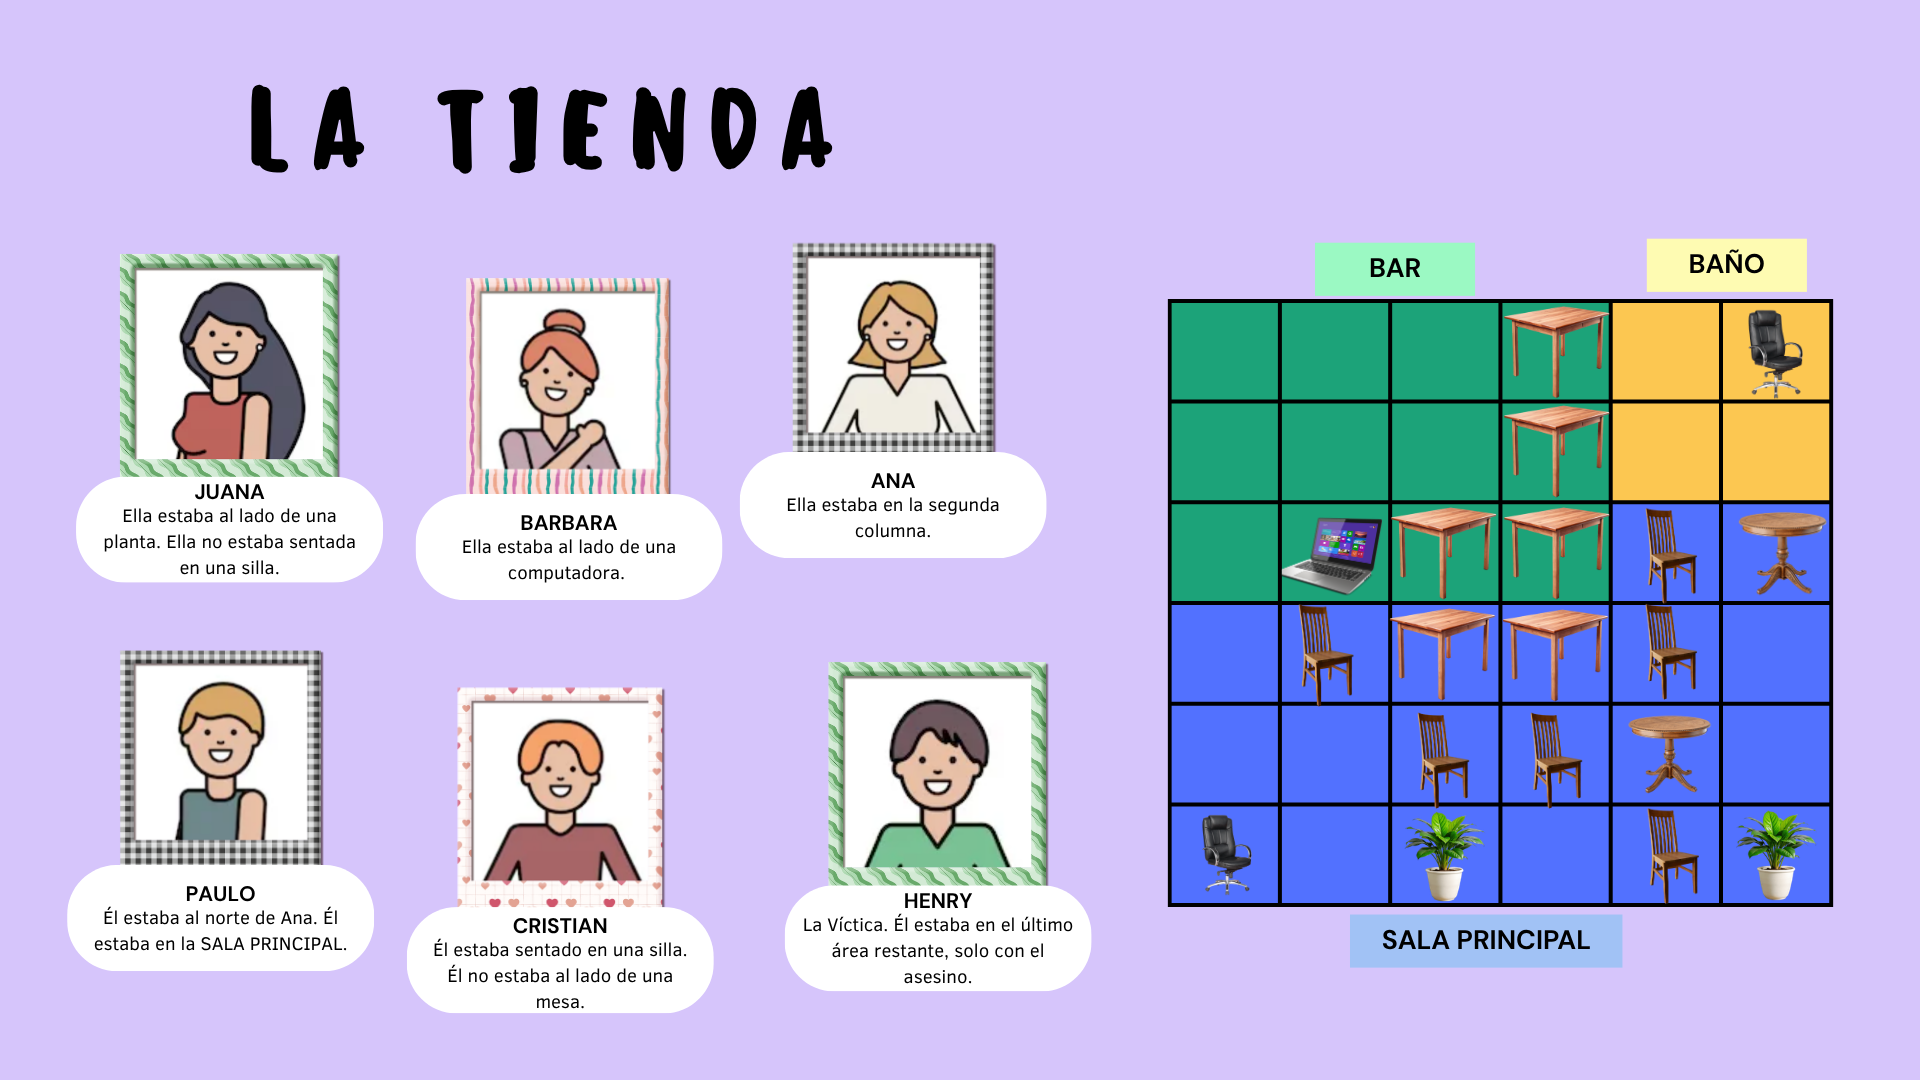
\includegraphics[width=\columnwidth]{la_tienda.png}
  \caption{Imagen de entrada del caso ``La Tienda'': seis tarjetas en una cuadrícula de
  $3\times2$ a la izquierda y el tablero rotulado a la derecha.}
  \label{fig:entrada}
\end{figure}

% =====================================================================
\section{Arquitectura del sistema}

El sistema está organizado en módulos independientes (Fig.~\ref{fig:pipeline}):
\begin{itemize}
  \item \texttt{src/vision.py}: Fase~1, extracción desde la imagen.
  \item \texttt{src/parser\_pistas.py}: traducción de testimonios a restricciones.
  \item \texttt{src/solver.py}: Fase~2, modelo CP-SAT, conteo de soluciones y diagnóstico.
  \item \texttt{src/visualizer.py}: Fase~3, proyección de la solución.
  \item \texttt{src/tutor.py} y \texttt{src/agent.py}: tutor interactivo basado en el
        solver, con redacción opcional por un LLM local.
  \item \texttt{src/catalogo.py} y \texttt{casos/casos.json}: catálogo de los 10 casos y su
        verdad de terreno.
  \item \texttt{main.py} (CLI) y \texttt{app.py} (API FastAPI e interfaz web).
\end{itemize}
El código incluye pruebas automáticas (\texttt{pytest}) del parser, el solver, el catálogo y
el tutor, y \emph{scripts} para validar el dataset y evaluar el \emph{pipeline}.

\begin{figure}[t]
\centering
\scriptsize
\setlength{\fboxsep}{3pt}
\fbox{\parbox{0.92\columnwidth}{\centering
\textbf{Imagen} (.png/.jpg)\\[2pt]
$\downarrow$\\
\textbf{Fase 1 -- Visión}: tablero (contornos) $\rightarrow$ $N$ (líneas) $\rightarrow$
celdas $\rightarrow$ habitaciones (K-Means CIELAB + OCR de etiquetas) $\rightarrow$
muebles (MobileNetV3 + coseno) $\rightarrow$ tarjetas (Tesseract)\\[2pt]
$\downarrow$\\
\textbf{Parser de testimonios} (reglas; LLM solo de respaldo)\\[2pt]
$\downarrow$ \texttt{puzzle\_data} (diccionario / JSON)\\[2pt]
\textbf{Fase 2 -- CP}: modelo CP-SAT $\rightarrow$ solución y verificación de unicidad\\[2pt]
$\downarrow$ posiciones $(X_p,Y_p,Z_p)$ y asesino\\[2pt]
\textbf{Fase 3}: superposición sobre el tablero / web / tutor
}}
\caption{\emph{Pipeline} end-to-end. Cada fase consume la salida de la anterior sin
intervención manual.}
\label{fig:pipeline}
\end{figure}

La estructura intermedia \texttt{puzzle\_data} es el contrato entre la visión y el solver:
\begin{lstlisting}
{ "N": 6,
  "sospechosos": ["Juana","Barbara","Ana","Paulo","Cristian"],
  "victima": "Henry",
  "habitaciones": {(r,c): id_sala, ...},
  "muebles": {"mesas": [(0,3),...], "sillas": [...],
              "plantas": [...], "computadora": [(2,1)]},
  "pistas": [{"tipo":"columna_fija","persona":"Ana","columna":1},
             {"tipo":"direccion_relativa","origen":"Paulo",
              "destino":"Ana","direccion":"norte"}, ...],
  "obstaculos": ["mesas","plantas","computadora"] }
\end{lstlisting}

% =====================================================================
\section{Fase 1: Visión Computacional e IA}

\subsection{Localización de la grilla}
La imagen se convierte a escala de grises y se binariza con umbral inverso ($T=60$), de modo
que el marco negro de la grilla queda en primer plano. Sobre la mitad derecha se extraen los
contornos externos con OpenCV~\cite{bradski2000opencv} y se elige el de mayor área que
supere el 20\,\% de la región y tenga razón de aspecto $w/h\in[0{,}8;\,1{,}2]$. El rectángulo
envolvente se recorta con un margen de 4\,px para eliminar el borde.

\subsection{Estimación de $N$ y segmentación de celdas}
Sobre el recorte se calcula la máscara de píxeles oscuros (gris $<60$) y sus perfiles de
proyección vertical y horizontal (fracción de píxeles oscuros por columna y por fila). Los
tramos con más del 60\,\% de píxeles oscuros son líneas; se descartan las pegadas al borde
(marco) y $N$ es el número de líneas internas más uno, aceptado solo si coincide en ambos
ejes. Con $N$, el recorte de $H\times W$ se divide en una malla regular de celdas de
$\lfloor H/N\rfloor\times\lfloor W/N\rfloor$ píxeles (Fig.~\ref{fig:segmentacion}).

\begin{figure}[t]
  \centering
  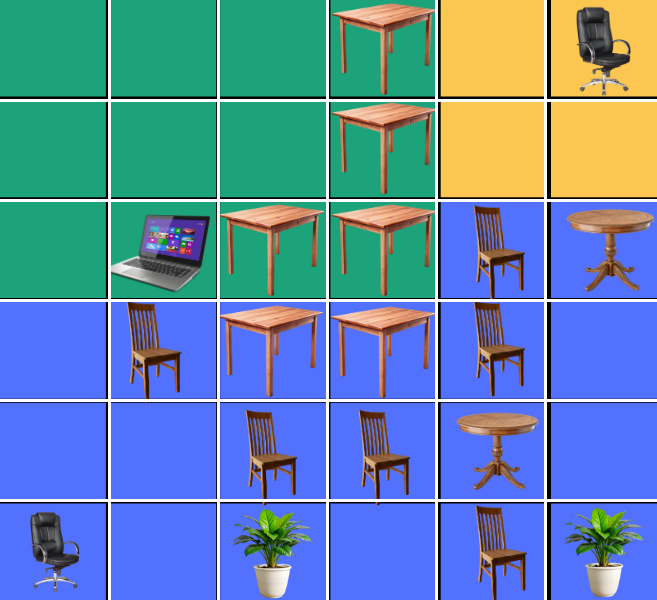
\includegraphics[width=0.62\columnwidth]{segmentacion.png}
  \caption{Grilla localizada y segmentada en $6\times6$ celdas.}
  \label{fig:segmentacion}
\end{figure}

\subsection{Segmentación y rotulado de habitaciones}
El color de fondo de cada celda se estima con la \emph{mediana} de los píxeles de sus
cuatro esquinas interiores (12\,\% del lado), lo que evita que el mueble central contamine
la estimación. Las muestras se convierten a CIELAB, espacio más cercano a la percepción
humana que RGB, y las $N^2$ medianas se agrupan con K-Means~\cite{lloyd1982}
($k$ = número de habitaciones, 10 inicializaciones).

Para saber \emph{qué} habitación es cada clúster ---necesario para pistas como ``estaba en la
Gerencia''--- se leen con Tesseract las etiquetas de color situadas encima y debajo del
tablero (\texttt{--psm 11}). Cada etiqueta se asocia a una sala por similitud de texto
(\texttt{difflib}, umbral 0,6) y aporta el matiz HSV de su color. Finalmente, las salas se
emparejan con los clústeres minimizando la distancia circular de matiz con el algoritmo
húngaro~\cite{kuhn1955}.

\subsection{Detección y clasificación de mobiliario}
\textbf{Detección de presencia.} Se descartan las celdas de suelo liso: si la desviación
estándar de la intensidad en la región central (64\,\% del área) es $\sigma<14$, la celda se
considera vacía.

\textbf{Clasificación por \emph{embeddings}.} De cada celda con objeto se extrae un vector
de características con MobileNetV3-Small~\cite{howard2019mobilenetv3} preentrenada en
ImageNet, reemplazando el clasificador por la identidad. El recorte se redimensiona a
$128\times128$, se normaliza con las estadísticas de ImageNet y produce un
\emph{embedding} $\mathbf{e}\in\mathbb{R}^{576}$ normalizado en $L_2$. Lo mismo se hace una
sola vez con 6 plantillas (dos sillas, dos mesas, planta y computadora). La clase asignada es
\begin{equation}
  \hat{k} = \arg\max_{t\in\mathcal{T}} \cos(\mathbf{e}_{\text{celda}},\mathbf{e}_t)
  \quad \text{si } \max_t \cos(\cdot) \geq 0{,}45 .
\end{equation}
Este enfoque \emph{one-shot} por similitud no requiere entrenamiento: un mueble nuevo se
agrega con una sola imagen de plantilla.

\subsection{Lectura de tarjetas y traducción de testimonios}
\textbf{OCR.} Las seis tarjetas ocupan cajas fijas, definidas en proporción a una imagen de
referencia de $1920\times1080$ y escaladas al tamaño real. Cada caja se pasa a gris, se
amplía $\times2$ con interpolación cúbica, se binariza con Otsu~\cite{otsu1979} y se lee con
Tesseract~\cite{smith2007tesseract} (modelo \texttt{spa}, \texttt{--psm 6}). El testimonio
empieza en la primera línea que arranca con ``Él/Ella/La''; el nombre es la palabra en
mayúsculas de la línea anterior. La víctima es la tarjeta que contiene ``la víctima''.

\textbf{Parser determinista.} Los testimonios usan un vocabulario cerrado, por lo que se
traducen con reglas sobre texto normalizado (minúsculas, sin tildes): expresiones regulares
para direcciones (``al norte de Ana''), ordinales de fila o columna (``segunda'',
``última''), adyacencia (``al lado de una planta''), sillas y nombres de salas, con
detección de negación (``no estaba''). Los nombres de personas se resuelven con
coincidencia difusa (\texttt{difflib}, umbral 0,75) para tolerar errores de OCR.

\textbf{Respaldo con LLM.} Solo las oraciones que ninguna regla reconoce se envían a un LLM
local (Llama~3.2 3B vía Ollama, temperatura 0, salida JSON). Su respuesta se valida
estrictamente (personas y salas existentes, índices dentro del tablero) antes de usarse. En
los 10 casos del dataset el respaldo no fue necesario.

\subsection{Dataset}
Se construyó un dataset de 10 casos originales (Tabla~\ref{tab:dataset}): 8 de $6\times6$ y
2 de $8\times8$, con tres habitaciones cada uno y de dificultad creciente. Su verdad de
terreno (mapa de salas, muebles, testimonios y culpable) está en \texttt{casos/casos.json};
un \emph{script} verifica con el solver que cada caso tenga solución única.

\begin{table}[t]
\centering
\caption{Dataset de casos}
\label{tab:dataset}
\begin{tabular}{llcc}
\toprule
\textbf{Caso} & \textbf{Dificultad} & $N$ & \textbf{Muebles}\\
\midrule
01 La Tienda              & Intermedio   & 6 & 19\\
02 La Oficina             & Principiante & 6 & 11\\
03 La Biblioteca Colonial & Principiante & 6 & 10\\
04 El Centro Tecnológico  & Intermedio   & 6 & 12\\
05 La Galería Minimalista & Intermedio   & 6 & 11\\
06 El Cafetín Universitario & Intermedio & 6 & 14\\
07 La Agencia de Diseño   & Avanzado     & 6 & 12\\
08 El Coworking Urbano    & Avanzado     & 6 & 12\\
09 La Mansión de Cristal  & Experto      & 8 & 17\\
10 La Sala de Prensa      & Experto      & 8 & 16\\
\bottomrule
\end{tabular}
\end{table}

\subsection{Métricas de la visión}
Para cada caso se mide:
\begin{itemize}
  \item \textbf{$N$}: la dimensión estimada coincide con la real.
  \item \textbf{Salas}: porcentaje de celdas con la habitación correcta.
  \item \textbf{Muebles}: una detección es acierto (TP) si coinciden tipo y celda;
        $\text{precisión}=\text{TP}/\text{detectados}$ y
        $\text{recall}=\text{TP}/\text{reales}$.
  \item \textbf{Nombres}: nombres de las 6 tarjetas leídos correctamente.
  \item \textbf{Pistas}: fracción de las pistas esperadas que se extrajeron.
\end{itemize}

La Fig.~\ref{fig:metricas} resume la evaluación completa del \emph{pipeline}
(\texttt{scripts/evaluar.py}). $N$ se estimó bien en los 10 casos, se leyeron los 60
nombres y el 100\,\% de las pistas esperadas, y en muebles se obtuvieron 133 aciertos sobre
135 detecciones y 134 muebles reales: precisión 98,5\,\% y \emph{recall} 99,3\,\%.

\begin{figure}[t]
  \centering
  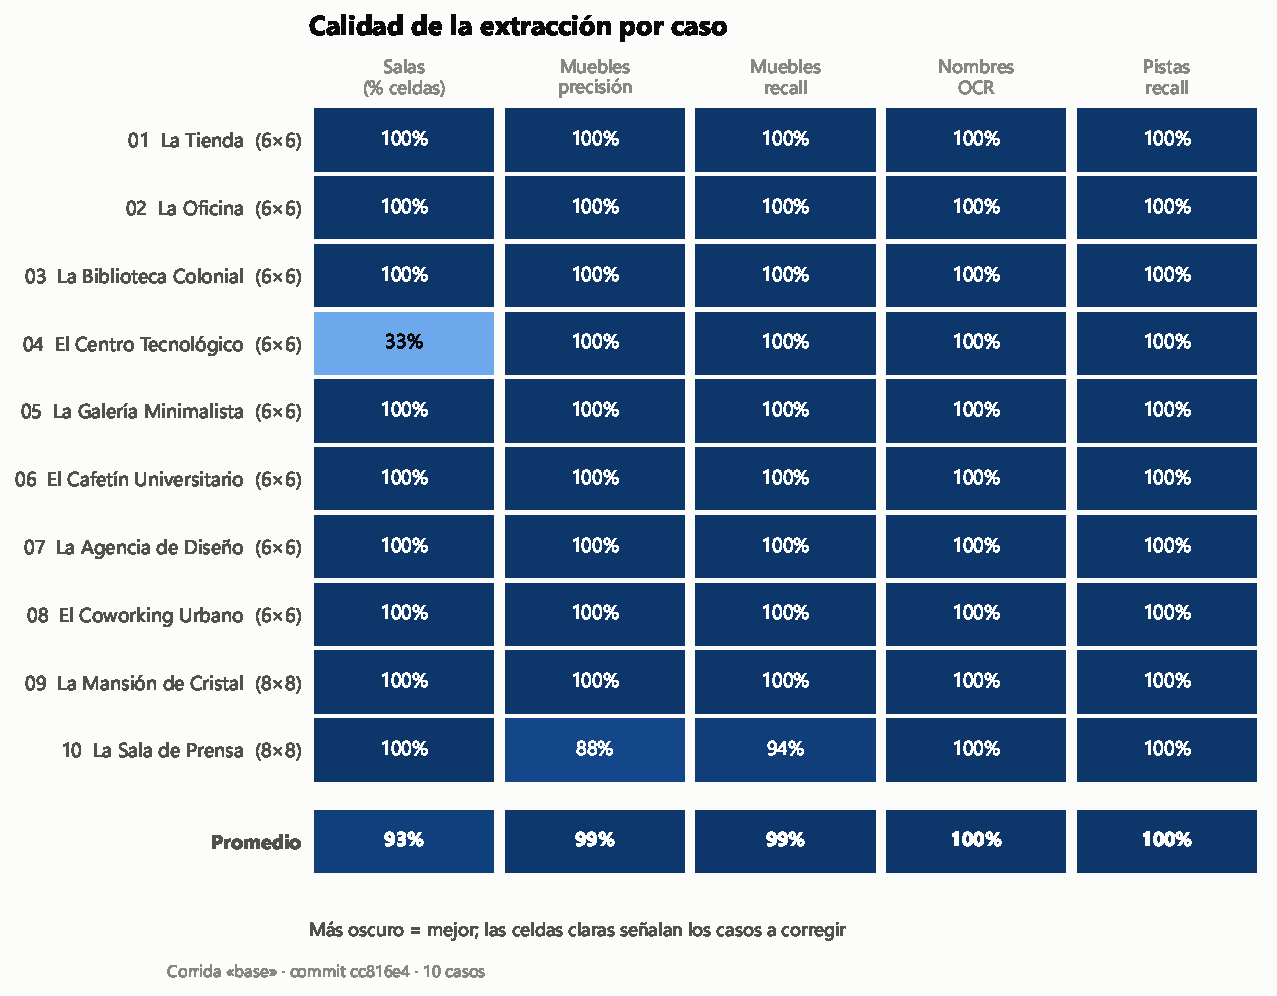
\includegraphics[width=\columnwidth]{fig_metricas_base.pdf}
  \caption{Calidad de la extracción por caso sobre las imágenes digitales.}
  \label{fig:metricas}
\end{figure}

\textbf{Análisis de errores.}
\begin{itemize}
  \item \emph{Caso 04, salas (33\,\%).} K-Means agrupa las celdas correctamente (100\,\%
        tomando la mejor correspondencia de etiquetas), pero el rotulado por color asignó
        nombres permutados a los clústeres. Con salas intercambiadas el modelo admite más de
        una solución, aunque el culpable obtenido sigue siendo el correcto.
  \item \emph{Caso 10, muebles.} Las tres discrepancias están en la última columna
        (Fig.~\ref{fig:caso10}). La inspección muestra que la imagen dibuja una planta en
        (3,7) y una silla en (5,7), con (6,7) vacía: la visión reporta lo que está dibujado y
        el error está en la imagen respecto al catálogo, no en el clasificador.
\end{itemize}

\begin{figure}[t]
  \centering
  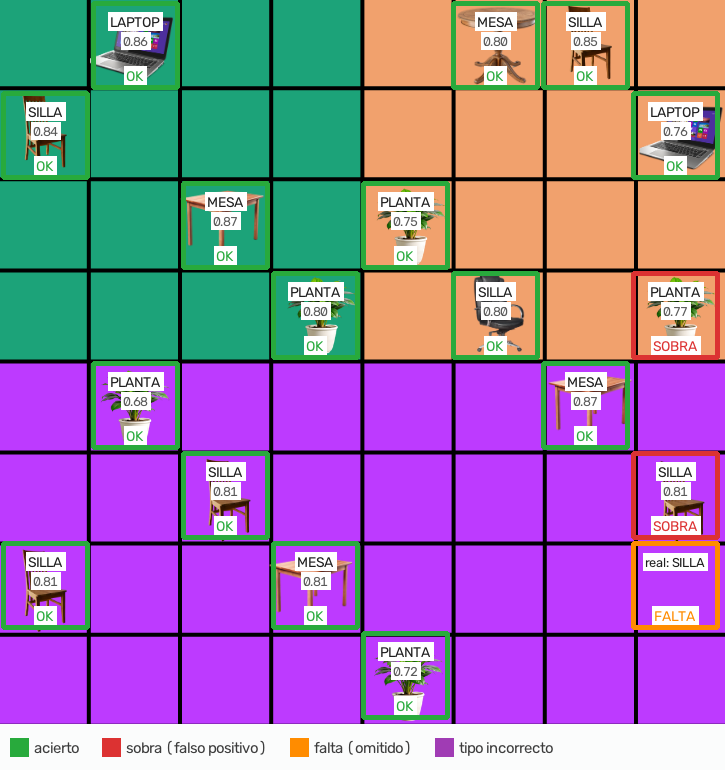
\includegraphics[width=0.85\columnwidth]{caso10_anotado.png}
  \caption{Detección por celda en el caso 10 con la similitud coseno de la plantilla
  ganadora. En rojo y naranja, las discrepancias con el catálogo.}
  \label{fig:caso10}
\end{figure}

\subsection{Robustez ante distintas condiciones de imagen}
Las imágenes del dataset son digitales. Para medir la robustez se generaron 10 variantes
de cada uno de los 10 casos que simulan condiciones de captura distintas
(Fig.~\ref{fig:variantes}), y se evaluaron las etapas de tablero, $N$, salas (K-Means) y
muebles: 110 imágenes en total. La Tabla~\ref{tab:robustez} muestra los resultados.

\begin{figure}[t]
  \centering
  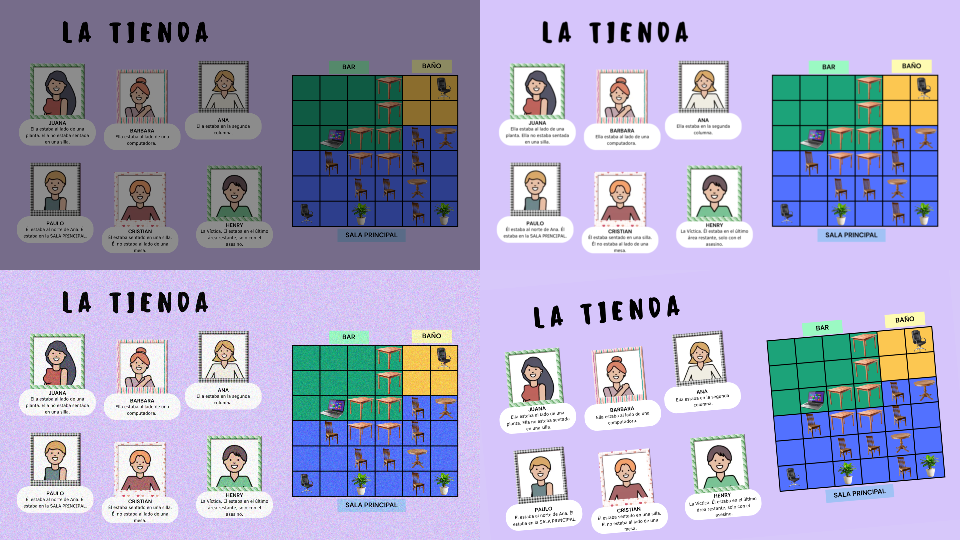
\includegraphics[width=\columnwidth]{variantes.png}
  \caption{Ejemplos de variantes: baja iluminación, desenfoque, ruido gaussiano y rotación
  de $5^\circ$.}
  \label{fig:variantes}
\end{figure}

\begin{table}[t]
\centering
\caption{Robustez de la visión (10 casos por condición)}
\label{tab:robustez}
\setlength{\tabcolsep}{4pt}
\begin{tabular}{lccccc}
\toprule
\textbf{Condición} & $N$ & \textbf{Salas} & \textbf{Prec.} & \textbf{Recall} & \textbf{Perf.}\\
\midrule
Original                    & 10/10 & 1,000 & 0,985 & 0,993 & 9\\
Oscura ($\alpha=0{,}55$)    & 10/10 & 1,000 & 0,983 & 0,843 & 1\\
Clara ($+50$)               & 10/10 & 1,000 & 0,985 & 0,993 & 9\\
Contraste ($\alpha=1{,}4$)  & 10/10 & 1,000 & 0,985 & 0,993 & 9\\
Desenfoque ($k=7$)          & 10/10 & 1,000 & 0,963 & 0,970 & 8\\
Ruido ($\sigma=20$)         & 10/10 & 1,000 & 0,985 & 0,955 & 6\\
JPEG (calidad 25)           & 10/10 & 1,000 & 0,985 & 0,993 & 9\\
Escala $0{,}5$              & 10/10 & 1,000 & 0,985 & 0,993 & 9\\
Perspectiva leve            &  0/10 & 0,997 & 0,985 & 0,993 & 8\\
Rotación $2^\circ$          &  0/10 & 0,869 & 0,985 & 0,993 & 1\\
Rotación $5^\circ$          &  0/10 & 0,797 & 0,715 & 0,918 & 0\\
\bottomrule
\multicolumn{6}{l}{\footnotesize Salas: mejor correspondencia de clústeres. Perf.: casos sin}\\
\multicolumn{6}{l}{\footnotesize ningún error de sala ni de mueble.}
\end{tabular}
\end{table}

El sistema es robusto a cambios de brillo y contraste, ruido, compresión, desenfoque y
cambio de escala. Las fallas son informativas:
\begin{itemize}
  \item \textbf{Baja iluminación}: los muebles perdidos no son errores de clasificación
        sino de \emph{detección}: con menos contraste, la desviación estándar del centro de
        la celda cae bajo el umbral fijo $\sigma=14$. Un umbral relativo a la imagen o una
        ecualización CLAHE previa lo corregiría.
  \item \textbf{Rotación y perspectiva}: las líneas de la grilla dejan de ser horizontales y
        el conteo de líneas por proyección falla (por eso $N$ se toma del catálogo en esos
        casos). Además, el recorte por rectángulo alineado a los ejes desfasa la malla, lo
        que produce errores de sala en los bordes y, a $5^\circ$, fragmentos de muebles
        vecinos detectados como falsos positivos. Se requiere una corrección de
        perspectiva con los cuatro vértices del contorno (\texttt{approxPolyDP} +
        \texttt{warpPerspective}).
\end{itemize}

% =====================================================================
\section{Fase 2: Modelo de Programación con Restricciones}

\subsection{Parámetros de la instancia}
Todos los parámetros provienen de \texttt{puzzle\_data}; el modelo no contiene datos de
ningún caso concreto:
\begin{itemize}
  \item $N$: dimensión de la grilla; $\mathcal{C}=\{0,\dots,N-1\}^2$ celdas.
  \item $\mathcal{S}$: sospechosos; $v$: víctima; $\mathcal{P}=\mathcal{S}\cup\{v\}$.
  \item $\mathcal{H}$: habitaciones; $\rho:\mathcal{C}\to\mathcal{H}$ mapa de habitaciones.
  \item $M_k\subseteq\mathcal{C}$: celdas con mueble de tipo $k$.
  \item $\mathcal{O}=\bigcup_{k\in K_{obs}} M_k$: celdas obstáculo (mesas, plantas,
        computadora).
  \item $\mathcal{A}(M)=\{(r',c')\in\mathcal{C} : |r-r'|+|c-c'|=1,\ (r,c)\in M\}$:
        vecindad ortogonal de un conjunto de celdas.
  \item $\Pi$: conjunto de pistas extraídas.
\end{itemize}

\subsection{Variables y dominios}
\begin{align}
  b_{p,r,c} &\in \{0,1\} && \forall p\in\mathcal{P},\ (r,c)\in\mathcal{C}\\
  X_p &\in \{0,\dots,N-1\} && \text{(fila de } p)\\
  Y_p &\in \{0,\dots,N-1\} && \text{(columna de } p)\\
  Z_p &\in \{\min\mathcal{H},\dots,\max\mathcal{H}\} && \text{(habitación de } p)\\
  \ell_k &\in \{0,1\} && \forall k\in\Pi \text{ (literal de pista)}
\end{align}
$b_{p,r,c}=1$ si y solo si $p$ ocupa la celda $(r,c)$. Además se usan booleanas auxiliares
$\nu_h$ y $\sigma_{s,h}$ para la regla del asesino (\S\ref{sec:reif}).

\subsection{Restricciones}

\textbf{(C1) Ocupación única} --- cada persona en exactamente una celda:
\begin{equation}
  \textstyle\sum_{(r,c)\in\mathcal{C}} b_{p,r,c} = 1 \qquad \forall p\in\mathcal{P}.
\end{equation}

\textbf{(C2--C3) Unicidad de filas y columnas}:
\begin{align}
  \textstyle\sum_{p\in\mathcal{P}}\sum_{c} b_{p,r,c} &\le 1 && \forall r,\\
  \textstyle\sum_{p\in\mathcal{P}}\sum_{r} b_{p,r,c} &\le 1 && \forall c.
\end{align}
Junto con (C1) y la canalización (C4), equivalen a las restricciones globales
\begin{equation}
  \AllDiff(X_p : p\in\mathcal{P}),\qquad \AllDiff(Y_p : p\in\mathcal{P}).
\end{equation}
Se expresan en su descomposición booleana \emph{at-most-one}, que CP-SAT reconoce y
propaga como restricción de cardinalidad mediante cláusulas y detección de
cliques~\cite{perron2023cpsat}. Esta codificación es eficiente porque la misma matriz $b$ se
reutiliza en las pistas sobre muebles, que se reducen a sumas lineales sin restricciones
\textsc{Element} adicionales.

\textbf{(C4) Canalización} (\emph{channeling}) entre la representación booleana y la
entera:
\begin{align}
  X_p &= \textstyle\sum_{(r,c)} r\, b_{p,r,c}, \qquad
  Y_p = \textstyle\sum_{(r,c)} c\, b_{p,r,c},\\
  Z_p &= \textstyle\sum_{(r,c)} \rho(r,c)\, b_{p,r,c} \qquad \forall p\in\mathcal{P}.
\end{align}
Dado (C1), (C4) implementa la restricción global
$Z_p = \textsc{Element}(\rho,\ \text{celda}(p))$ como una suma lineal.

\textbf{(C5) Obstáculos}:
\begin{equation}
  b_{p,r,c} = 0 \qquad \forall p\in\mathcal{P},\ (r,c)\in\mathcal{O}.
\end{equation}

\textbf{(C6) Regla del asesino} (reificada): si la víctima está en $h$, exactamente un
sospechoso está en $h$:
\begin{align}
  \nu_h &\Leftrightarrow (Z_v = h) && \forall h\in\mathcal{H},\\
  \sigma_{s,h} &\Leftrightarrow (Z_s = h) && \forall s\in\mathcal{S},\ h\in\mathcal{H},\\
  \nu_h &\Rightarrow \textstyle\sum_{s\in\mathcal{S}} \sigma_{s,h} = 1 && \forall h\in\mathcal{H}.
\end{align}
El asesino es el único $s$ con $Z_s=Z_v$.

\textbf{(C7) Pistas} (semirreificadas): cada pista $k\in\Pi$ se traduce a una restricción
$R_k$ según la Tabla~\ref{tab:pistas} y se condiciona a su literal:
\begin{equation}
  \ell_k \Rightarrow R_k \qquad \forall k\in\Pi.
\end{equation}
Al resolver un caso se fija $\ell_k=1$ para toda pista. Un tipo de pista, persona, sala o
dirección desconocida produce un error explícito en lugar de ignorarse, porque omitir una
pista en silencio podría devolver una solución incorrecta.

\begin{table}[t]
\centering
\caption{Traducción de pistas a restricciones $R_k$}
\label{tab:pistas}
\begin{tabular}{ll}
\toprule
\textbf{Tipo de pista} & \textbf{Restricción}\\
\midrule
\texttt{columna\_fija}$(p,j)$ & $Y_p = j$\\
\texttt{fila\_fija}$(p,i)$ & $X_p = i$\\
\texttt{habitacion\_fija}$(p,h)$ & $Z_p = h$\\
\texttt{direccion}$(p,q,\text{norte})$ & $X_p < X_q$\\
\texttt{direccion}$(p,q,\text{sur})$ & $X_p > X_q$\\
\texttt{direccion}$(p,q,\text{este})$ & $Y_p > Y_q$\\
\texttt{direccion}$(p,q,\text{oeste})$ & $Y_p < Y_q$\\
\texttt{sobre\_objeto}$(p,k)$ & $\sum_{(r,c)\in M_k} b_{p,r,c} = 1$\\
\texttt{no\_sobre\_objeto}$(p,k)$ & $\sum_{(r,c)\in M_k} b_{p,r,c} = 0$\\
\texttt{adyacente\_a}$(p,k)$ & $\sum_{(r,c)\in\mathcal{A}(M_k)} b_{p,r,c} \ge 1$\\
\texttt{no\_adyacente\_a}$(p,k)$ & $\sum_{(r,c)\in\mathcal{A}(M_k)} b_{p,r,c} = 0$\\
\bottomrule
\end{tabular}
\end{table}

\subsection{Uso de restricciones reificadas}\label{sec:reif}
La reificación se usa en dos lugares, cada uno por una razón concreta:

\textbf{Regla del asesino (C6).} Es \emph{condicional} a una decisión del propio modelo
---la habitación de la víctima---, por lo que no puede expresarse como restricción dura
fija. Se implementa con literales de activación (\texttt{OnlyEnforceIf}) de CP-SAT en
ambos sentidos.

\textbf{Pistas (C7).} Para resolver, todas las pistas son hechos ciertos y bastaría
imponerlas como restricciones duras; fijar $\ell_k=1$ hace que la presolución las elimine,
sin costo de propagación. La reificación aporta valor en el \textbf{modo tutor}: las
ubicaciones del jugador se agregan como literales $m_{p}=b_{p,r,c}$ y, junto con los
$\ell_k$, se pasan al solver como \emph{supuestos} (\texttt{AddAssumptions}). Si el
modelo es infactible, CP-SAT devuelve un subconjunto de supuestos suficiente para la
contradicción (\texttt{SufficientAssumptionsForInfeasibility}), es decir, qué
ubicaciones y qué testimonios chocan, lo que se muestra al jugador sin revelar la solución.
Las pistas se reifican solo en un sentido ($\ell_k\Rightarrow R_k$), porque no se necesita
deducir que una pista es falsa.

El tutor también usa el modelo para calcular las celdas factibles de la persona más
acotada (una resolución con un supuesto por celda candidata) y ofrecer ayuda progresiva en
tres niveles.

\subsection{Implementación en OR-Tools CP-SAT}\label{sec:codigo}
El modelo se construye en la función \texttt{\_construir\_modelo()} de
\texttt{src/solver.py}. Cada restricción formal corresponde a una o pocas líneas de la API
de CP-SAT; los listados siguientes reproducen el código con nombres abreviados.
El Listado~\ref{lst:globales} muestra las variables y las restricciones estructurales
(C1--C5). Todos los rangos y conjuntos ($N$, personas, mapa de salas, muebles) se leen de
\texttt{puzzle\_data}, por lo que el mismo código sirve para cualquier instancia.

\begin{lstlisting}[language=Python,caption={Variables y restricciones C1--C5},label={lst:globales}]
model = cp_model.CpModel()
celdas = [(r, c) for r in range(N) for c in range(N)]

# Booleanas de ocupacion b[p,r,c]
celda = {(p, r, c): model.NewBoolVar(f"celda_{p}_{r}_{c}")
         for p in range(P) for (r, c) in celdas}

# C1: cada persona en exactamente una celda
for p in range(P):
    model.Add(sum(celda[p, r, c] for r, c in celdas) == 1)

# C2-C3: AllDifferent en filas y columnas (at-most-one)
for r in range(N):
    model.Add(sum(celda[p, r, c] for p in range(P)
                  for c in range(N)) <= 1)
for c in range(N):
    model.Add(sum(celda[p, r, c] for p in range(P)
                  for r in range(N)) <= 1)

# C4: canalizacion a fila X, columna Y y habitacion Z
X = [model.NewIntVar(0, N - 1, f"X_{p}") for p in personas]
Y = [model.NewIntVar(0, N - 1, f"Y_{p}") for p in personas]
Z = [model.NewIntVar(min(ids_hab), max(ids_hab), f"Z_{p}")
     for p in personas]
for p in range(P):
    model.Add(X[p] == sum(r * celda[p, r, c] for r, c in celdas))
    model.Add(Y[p] == sum(c * celda[p, r, c] for r, c in celdas))
    model.Add(Z[p] == sum(mapa_hab[r, c] * celda[p, r, c]
                          for r, c in celdas))

# C5: obstaculos (mesas, plantas, computadora)
for tipo in obstaculos:
    for r, c in muebles.get(tipo, []):
        for p in range(P):
            model.Add(celda[p, r, c] == 0)
\end{lstlisting}

El Listado~\ref{lst:reif} muestra las restricciones reificadas. En CP-SAT la reificación se
expresa con \texttt{OnlyEnforceIf(lit)}: la restricción solo se exige cuando el literal
\texttt{lit} es verdadero. Para la regla del asesino (C6) se reifica la igualdad
$Z_v=h$ en ambos sentidos; para las pistas (C7), cada una recibe su literal $\ell_k$, que
se fija a 1 al resolver o se pasa como supuesto en el modo tutor.

\begin{lstlisting}[language=Python,caption={Restricciones reificadas C6--C7 y diagnóstico},label={lst:reif}]
# C6: victima en h  =>  exactamente un sospechoso en h
for h in ids_hab:
    vic_en_h = model.NewBoolVar(f"vic_en_hab_{h}")
    model.Add(Z[v] == h).OnlyEnforceIf(vic_en_h)
    model.Add(Z[v] != h).OnlyEnforceIf(vic_en_h.Not())
    s_en_h = []
    for s in range(S):
        b = model.NewBoolVar(f"s_{s}_en_hab_{h}")
        model.Add(Z[s] == h).OnlyEnforceIf(b)
        model.Add(Z[s] != h).OnlyEnforceIf(b.Not())
        s_en_h.append(b)
    model.Add(sum(s_en_h) == 1).OnlyEnforceIf(vic_en_h)

# C7: cada pista k condicionada a su literal l_k
for pista in pistas:
    lit = model.NewBoolVar(f"pista_{k}")
    if pista["tipo"] == "columna_fija":
        model.Add(Y[p] == pista["columna"]).OnlyEnforceIf(lit)
    elif pista["tipo"] == "direccion_relativa":  # norte
        model.Add(X[o] < X[d]).OnlyEnforceIf(lit)
    elif pista["tipo"] == "adyacente_a":
        vec = vecinos_de(muebles[pista["objeto"]], N)
        model.Add(sum(celda[p, r, c] for r, c in vec) >= 1
                  ).OnlyEnforceIf(lit)
    # ... resto de tipos de la Tabla de pistas

# Resolver: todas las pistas activas
for lit in literales:
    model.Add(lit == 1)

# Tutor: pistas y jugadas como supuestos
model.AddAssumptions(literales + jugadas)
if solver.Solve(model) == cp_model.INFEASIBLE:
    nucleo = solver.SufficientAssumptionsForInfeasibility()
\end{lstlisting}

Además de \texttt{resolver\_murdoku()}, el módulo ofrece \texttt{contar\_soluciones()}, que
enumera soluciones con \texttt{enumerate\_all\_solutions} y un \emph{callback} para
verificar la unicidad de cada caso, y \texttt{celdas\_factibles()}, que el tutor usa para
calcular dónde puede estar cada persona.

\subsection{Solución del caso ``La Tienda''}
La Tabla~\ref{tab:solucion} muestra las posiciones obtenidas: Barbara es la única
sospechosa en el Bar junto a Henry, por lo que es la asesina.

\begin{table}[t]
\centering
\caption{Solución del caso ``La Tienda'' (índices desde 0)}
\label{tab:solucion}
\begin{tabular}{lccl}
\toprule
\textbf{Persona} & \textbf{Fila} & \textbf{Col.} & \textbf{Habitación}\\
\midrule
Juana    & 5 & 3 & Sala Principal\\
Barbara  & 2 & 0 & Bar \textbf{(asesina)}\\
Ana      & 4 & 1 & Sala Principal\\
Paulo    & 3 & 4 & Sala Principal\\
Cristian & 0 & 5 & Baño\\
Henry    & 1 & 2 & Bar (víctima)\\
\bottomrule
\end{tabular}
\end{table}

% =====================================================================
\section{Análisis de complejidad y tiempos}

\subsection{Tamaño del espacio de búsqueda}
Sin restricciones, colocar $|\mathcal{P}|$ personas en $N^2$ celdas da
$(N^2)^{|\mathcal{P}|}$ configuraciones: para $N=|\mathcal{P}|=6$ son
$36^6\approx2{,}18\times10^9$. Las restricciones (C1--C3) lo reducen a las asignaciones
inyectivas de filas y columnas, $\left(\frac{N!}{(N-|\mathcal{P}|)!}\right)^2$: para $N=6$
son $(6!)^2=518\,400$ y para $N=8$, $(8!/2!)^2\approx4{,}06\times10^8$. Con obstáculos y la
regla del asesino, pero sin pistas, los casos de $6\times6$ aún tienen entre 7\,680 y
123\,840 soluciones (Tabla~\ref{tab:casos}); las pistas las reducen a una.

El problema general de satisfacción de restricciones es NP-completo~\cite{rossi2006handbook},
por lo que no se espera un algoritmo polinomial para la familia generalizada. Sin embargo,
los Murdoku están diseñados para resolverse por deducción, lo que favorece a la propagación.

\subsection{Tamaño del modelo}
El número de variables es
\begin{equation}
  |V| = \underbrace{|\mathcal{P}|N^2}_{b} + \underbrace{3|\mathcal{P}|}_{X,Y,Z}
        + \underbrace{|\mathcal{H}|(1+|\mathcal{S}|)}_{\nu,\sigma} + \underbrace{|\Pi|}_{\ell}
  = O(|\mathcal{P}|N^2),
\end{equation}
que para ``La Tienda'' da $216+18+18+8=260$ variables, como reporta el modelo generado. El
número de restricciones es $O(N+|\mathcal{P}||\mathcal{H}|+|\Pi|)$, pero (C2--C4)
involucran $O(|\mathcal{P}|N)$ y $O(N^2)$ literales cada una, de modo que el tamaño total
del modelo es $O(|\mathcal{P}|N^2)$.

\subsection{Tiempos de respuesta}
Las mediciones se hicieron en un Intel Core i5-6500 (3,2\,GHz, 4 núcleos) con 20\,GB de RAM,
Windows~10, Python~3.13 y OR-Tools~9.15 con parámetros por defecto.

La Tabla~\ref{tab:casos} resume el solver sobre los 10 casos (30 ejecuciones cada uno).
Todos tienen solución única, el culpable coincide con el del catálogo y \textbf{ninguno
requiere ramificación}: la presolución y la propagación fijan todas las variables. El
tiempo reportado por CP-SAT está entre 9 y 22~ms, y el tiempo total, incluida la
construcción del modelo en Python, entre 17 y 35~ms.

\begin{table}[t]
\centering
\caption{Solver sobre los 10 casos del dataset}
\label{tab:casos}
\setlength{\tabcolsep}{3pt}
\begin{tabular}{lrrrrrr}
\toprule
\textbf{Caso} & $|V|$ & \textbf{Restr.} & $|\Pi|$ & \textbf{Nec.} & \textbf{Sol. sin $\Pi$} & \textbf{t (ms)}\\
\midrule
01 & 260 & 157 &  8 &  3 &   7\,680 & 13,7\\
02 & 264 & 141 & 12 &  4 &  43\,680 & 22,3\\
03 & 264 & 141 & 12 &  5 &  44\,400 & 14,6\\
04 & 262 & 143 & 10 &  7 & 123\,840 & 16,0\\
05 & 261 & 135 &  9 &  5 &  11\,520 & 13,2\\
06 & 264 & 153 & 12 &  4 &  92\,160 & 12,9\\
07 & 264 & 147 & 12 &  5 &  36\,480 & 11,2\\
08 & 261 & 135 &  9 &  5 &  20\,160 &  9,1\\
09 & 434 & 173 & 14 & 10 & $>$167\,487 & 20,1\\
10 & 435 & 169 & 15 & 10 & $>$194\,276 & 18,2\\
\bottomrule
\multicolumn{7}{l}{\footnotesize Nec.: pistas cuya eliminación rompe la unicidad. Sol. sin $\Pi$:}\\
\multicolumn{7}{l}{\footnotesize soluciones sin pistas ($>$: enumeración cortada a 60\,s).}\\
\multicolumn{7}{l}{\footnotesize t: tiempo medio de CP-SAT. Todos: 0 ramas y 0 conflictos.}
\end{tabular}
\end{table}

\textbf{Ablación de pistas.} La columna ``Nec.'' indica cuántas pistas son imprescindibles:
al eliminar cualquiera de ellas aparece más de una solución. En los casos de $6\times6$ solo
entre 3 y 7 pistas lo son; el resto son redundantes dadas las demás, lo que es propio de un
acertijo diseñado con varias rutas de deducción. En los casos ``Experto'' de $8\times8$, 10
de las 14--15 pistas son necesarias.

\textbf{Escalabilidad.} Para medir el crecimiento se generaron instancias sintéticas de
$N\times N$ con $|\mathcal{P}|=N$ personas, 3 habitaciones y una pista
(Tabla~\ref{tab:escala} y Fig.~\ref{fig:escala}, 10 ejecuciones). El crecimiento es
polinomial en la práctica, dominado por el tamaño $O(N^3)$ del modelo cuando
$|\mathcal{P}|=N$: incluso con $30\times30$ y 27\,181 variables se resuelve en unos 10~s.

\begin{table}[t]
\centering
\caption{Escalabilidad del modelo ($|\mathcal{P}|=N$)}
\label{tab:escala}
\begin{tabular}{rrrr}
\toprule
$N$ & \textbf{Variables} & \textbf{Restricciones} & \textbf{Tiempo (ms)}\\
\midrule
4  & 89      & 53  & $17{,}5\pm2{,}5$\\
6  & 253     & 77  & $34{,}3\pm3{,}2$\\
8  & 561     & 101 & $71{,}9\pm7{,}1$\\
10 & 1\,061  & 125 & $146{,}4\pm11{,}1$\\
12 & 1\,801  & 149 & $302{,}3\pm17{,}8$\\
15 & 3\,466  & 185 & $779{,}2\pm11{,}4$\\
20 & 8\,121  & 245 & $3\,021\pm39$\\
25 & 15\,776 & 305 & $5\,908\pm152$\\
30 & 27\,181 & 365 & $10\,615\pm588$\\
\bottomrule
\end{tabular}
\end{table}

\begin{figure}[t]
\centering
\begin{tikzpicture}
\begin{axis}[
  width=\columnwidth, height=5cm,
  xlabel={$N$}, ylabel={Tiempo (ms)},
  ymode=log, grid=major,
  xtick={4,6,8,10,12,15,20,25,30},
  tick label style={font=\scriptsize},
  label style={font=\small}
]
\addplot[mark=*, thick, blue] coordinates {
  (4,17.5) (6,34.3) (8,71.9) (10,146.4) (12,302.3)
  (15,779.2) (20,3021.1) (25,5907.7) (30,10614.8)};
\end{axis}
\end{tikzpicture}
\caption{Tiempo total de construcción y resolución en función de $N$ (escala logarítmica).}
\label{fig:escala}
\end{figure}

\textbf{Costo del \emph{pipeline} completo.} La Fig.~\ref{fig:tiempos} muestra los tiempos
de la evaluación completa por caso: la visión con OCR toma entre 2,2 y 3,0~s y el solver
entre 9 y 26~ms. De la visión, la localización y K-Means toman unos 20~ms y la extracción de
\emph{embeddings} entre 120 y 350~ms en CPU; el resto corresponde a Tesseract. El solver
representa menos del 1\,\% del tiempo total.

\begin{figure}[t]
  \centering
  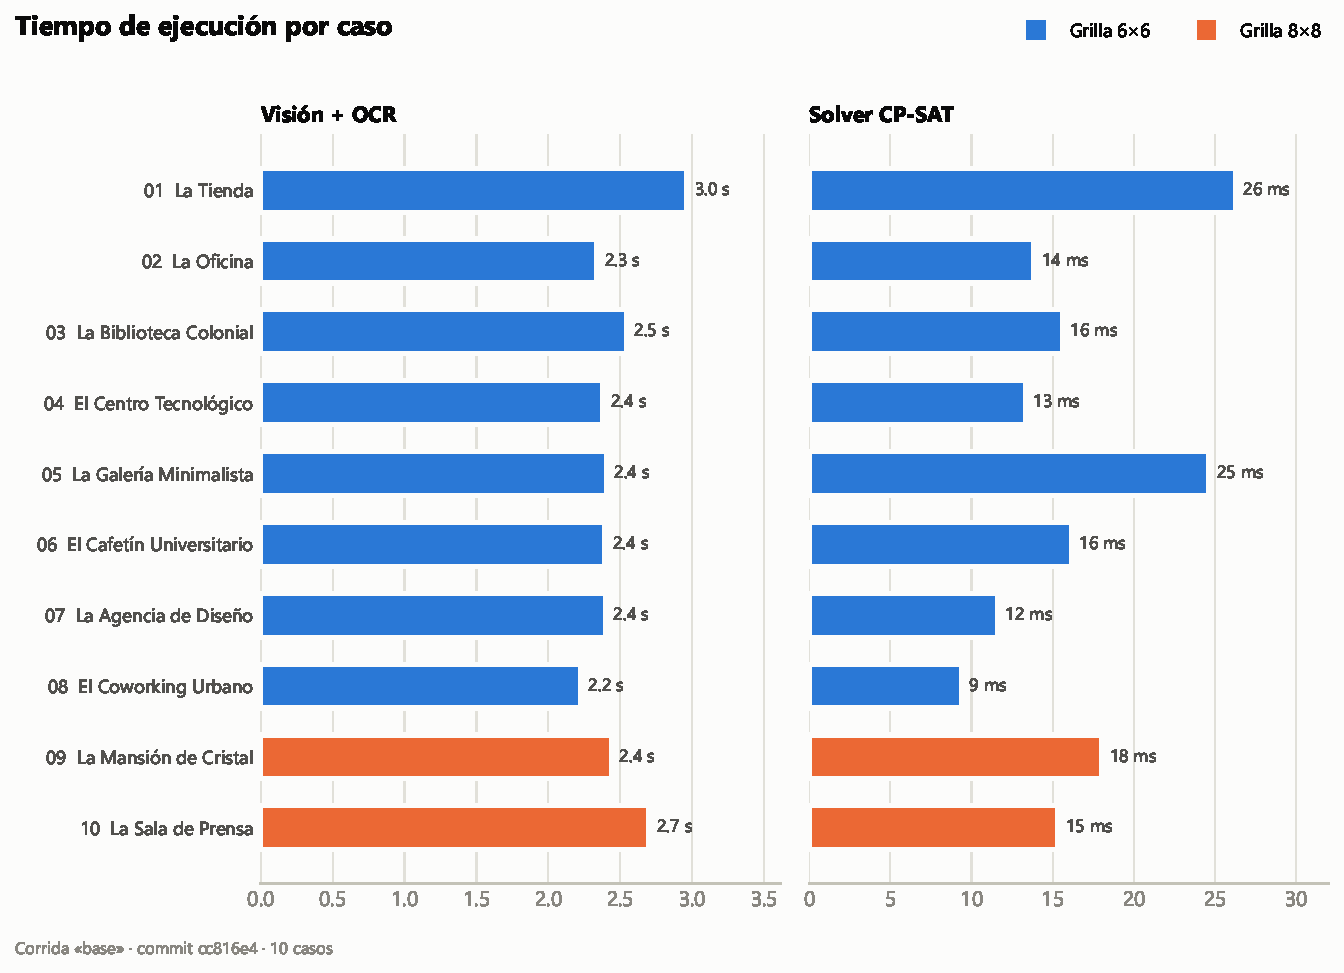
\includegraphics[width=\columnwidth]{fig_tiempos_base.pdf}
  \caption{Tiempo de visión + OCR y de CP-SAT por caso.}
  \label{fig:tiempos}
\end{figure}

% =====================================================================
\section{Fase 3: Integración y visualización}

La integración es automática: \texttt{extraer\_puzzle\_completo()} devuelve
\texttt{puzzle\_data}, que \texttt{resolver\_murdoku()} consume directamente, y su resultado
alimenta a \texttt{dibujar\_solucion\_sobre\_tablero()}. El usuario solo elige la imagen.

La solución se proyecta sobre el recorte original del tablero (Fig.~\ref{fig:solucion}):
cada persona se marca con un rectángulo semitransparente (opacidad 45\,\%, para que el color
de la habitación siga visible) y su nombre; el asesino se resalta en rojo con borde grueso y
la víctima en gris oscuro.

\begin{figure}[t]
  \centering
  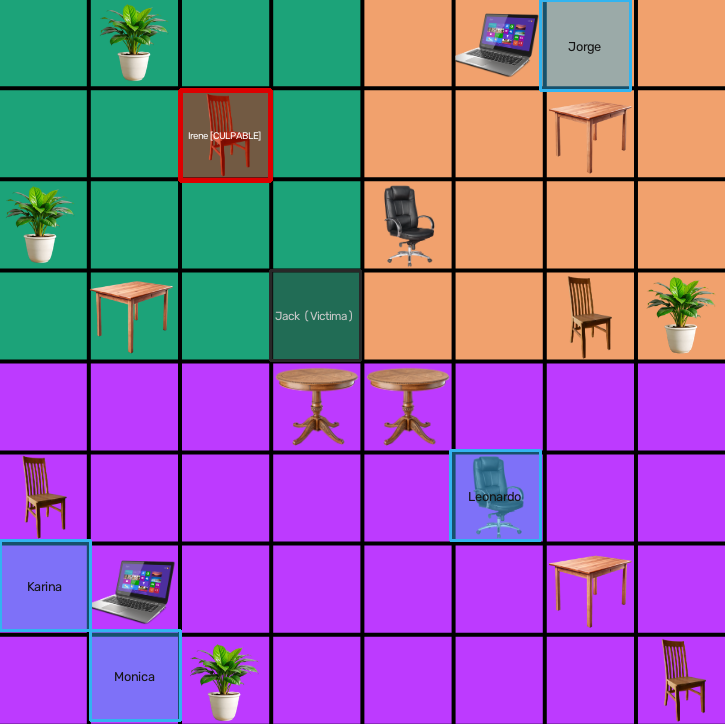
\includegraphics[width=0.85\columnwidth]{resuelto_caso_09.png}
  \caption{Solución del caso 09 ($8\times8$) proyectada sobre la imagen original. En rojo,
  la asesina (Irene); en gris, la víctima.}
  \label{fig:solucion}
\end{figure}

El sistema se ofrece en dos modos:
\begin{itemize}
  \item \textbf{CLI} (\texttt{python main.py --caso caso\_02}): ejecuta el \emph{pipeline},
        imprime lo extraído, indica si la solución es única y guarda la imagen resuelta.
  \item \textbf{Web} (\texttt{python app.py}): API REST con FastAPI (\texttt{/api/casos},
        \texttt{/api/analizar}, \texttt{/api/resolver}, \texttt{/api/tutor},
        \texttt{/api/validar}) y una interfaz con galería de casos y tablero interactivo. El
        jugador ubica personas, el solver valida su avance (\S\ref{sec:reif}) y ofrece
        pistas progresivas; opcionalmente, un LLM local reformula el mensaje, y una guardia
        descarta su texto si agrega números, nombres o razonamiento nuevos.
\end{itemize}

% =====================================================================
\section{Discusión y limitaciones}

\begin{itemize}
  \item \textbf{Corrección de perspectiva.} La localización usa el rectángulo envolvente
        alineado a los ejes y el conteo de líneas por proyección, suficientes para imágenes
        digitales y fotos frontales, pero no para rotaciones o perspectiva
        (Tabla~\ref{tab:robustez}). La mejora directa es una transformación de cuatro puntos
        sobre el contorno de la grilla.
  \item \textbf{Umbral de detección fijo.} El umbral $\sigma=14$ falla con poca luz y debe
        hacerse adaptativo.
  \item \textbf{Información del catálogo.} La CLI y la evaluación pasan $N$ y la lista de
        nombres de salas del catálogo. $N$ se estimó correctamente en las 10 imágenes
        digitales, por lo que podría tomarse siempre de la imagen; los nombres de sala sirven
        como vocabulario para rotular clústeres e interpretar pistas, y sin ellos las salas
        se numeran por color.
  \item \textbf{Diseño fijo de tarjetas.} Las cajas de las tarjetas son proporciones fijas
        del diseño del dataset; otro diseño requeriría detectarlas por contornos.
  \item \textbf{Dataset.} Las variantes de robustez son sintéticas; deben complementarse con
        fotografías de versiones impresas.
\end{itemize}

% =====================================================================
\section{Conclusiones}

Se desarrolló un sistema \emph{end-to-end} que lee la imagen de un Murdoku y lo resuelve
sin intervención manual. Sin entrenar ninguna red, la combinación de K-Means en CIELAB,
\emph{embeddings} de MobileNetV3, Tesseract y un parser determinista extrajo correctamente
los nombres y las pistas de los 10 casos, con 98,5\,\% de precisión y 99,3\,\% de
\emph{recall} en muebles, y el sistema identificó al culpable correcto en todos. El modelo
CP, con representación booleana canalizada a coordenadas enteras, restricciones \AllDiff{}
y reificación donde aporta ---la regla del asesino y el diagnóstico de errores del
jugador---, resolvió cada caso en 9--22~ms solo por propagación y escala a grillas de
$30\times30$ en segundos. El cuello de botella no es el solver sino la percepción: el
trabajo futuro debe centrarse en la corrección de perspectiva, umbrales adaptativos y un
dataset de fotografías reales.

% =====================================================================
\begin{thebibliography}{10}

\bibitem{rossi2006handbook}
F.~Rossi, P.~van Beek y T.~Walsh, Eds., \emph{Handbook of Constraint Programming}.
Amsterdam: Elsevier, 2006.

\bibitem{ortools}
L.~Perron y V.~Furnon, ``OR-Tools,'' Google, 2024. [En línea]. Disponible:
\url{https://developers.google.com/optimization}

\bibitem{perron2023cpsat}
L.~Perron, F.~Didier y S.~Gay, ``The CP-SAT-LP solver,'' en \emph{Proc. 29th Int. Conf.
Principles and Practice of Constraint Programming (CP 2023)}, LIPIcs, vol.~280, 2023,
pp.~3:1--3:2.

\bibitem{murdoku}
``Murdoku,'' \emph{Wikipedia}. [En línea]. Disponible:
\url{https://nl.wikipedia.org/wiki/Murdoku}

\bibitem{howard2019mobilenetv3}
A.~Howard \emph{et al.}, ``Searching for MobileNetV3,'' en \emph{Proc. IEEE/CVF Int.
Conf. Computer Vision (ICCV)}, 2019, pp.~1314--1324.

\bibitem{lloyd1982}
S.~Lloyd, ``Least squares quantization in PCM,'' \emph{IEEE Trans. Inf. Theory}, vol.~28,
no.~2, pp.~129--137, 1982.

\bibitem{kuhn1955}
H.~W.~Kuhn, ``The Hungarian method for the assignment problem,'' \emph{Naval Research
Logistics Quarterly}, vol.~2, no.~1--2, pp.~83--97, 1955.

\bibitem{otsu1979}
N.~Otsu, ``A threshold selection method from gray-level histograms,'' \emph{IEEE Trans.
Syst., Man, Cybern.}, vol.~9, no.~1, pp.~62--66, 1979.

\bibitem{smith2007tesseract}
R.~Smith, ``An overview of the Tesseract OCR engine,'' en \emph{Proc. 9th Int. Conf.
Document Analysis and Recognition (ICDAR)}, 2007, pp.~629--633.

\bibitem{bradski2000opencv}
G.~Bradski, ``The OpenCV library,'' \emph{Dr. Dobb's Journal of Software Tools}, 2000.

\end{thebibliography}

\end{document}
